\documentclass{beamer}
\usepackage[utf8]{inputenc}
\usepackage[inline]{enumitem}
\usepackage{pdfpages}
\usepackage{listings}
\usepackage{subcaption}
\usepackage{wasysym}
\usepackage[export]{adjustbox}[2011/08/13]
\usetheme{cern}

\newcommand{\btVFill}{\vskip0pt plus 1filll}

% fix tilde
% \newcommand{\propertilde}{\raise.17ex\hbox{$\scriptstyle\mathtt{\sim}$}}

% \setbeameroption{show notes on second screen=right}

%The CERN logo is legally protected. Please visit http://cern.ch/copyright for
%information on the terms of use of CERN content, including the CERN logo.

% The optional `\author` command defines the author and is displayed in the
%slide produced by the `\titlepage` command.
\author{Corné Lukken, Giulia Frascaria \& Animesh Trivedi}

% The optional `\title` command defines the title and is displayed in the slide
%produced by the `\titlepage` command.
\title{ZCSD: a Computational Storage Device over Zoned Namespaces SSDs}

% The optional `\subtitle` command will add a smaller title below the main one,
%and will not be displayed in any of the slides' footer.
% \subtitle{A SPDK compared to lightnvm story}

% The optional `\date` command will display a custom free text date on the all
%of the slides' footer. If omitted today's date will be used.
%\date{Monday, 1st January 2018}

% ------------------------------------------------------------------------%
% Proper Python Syntax Highlighting                                       %
% Author: redmode
% https://tex.stackexchange.com/questions/83882/how-to-highlight-python   %
% -syntax-in-latex-listings-lstinputlistings-command#83883                %
% ----------------------------------------------------------------------- %

% Default fixed font does not support bold face
\DeclareFixedFont{\ttb}{T1}{txtt}{bx}{n}{6} % for bold
\DeclareFixedFont{\ttm}{T1}{txtt}{m}{n}{6}  % for normal

% Custom colors
\definecolor{deepblue}{rgb}{0,0,0.5}
\definecolor{deepred}{rgb}{0.6,0,0}
\definecolor{deepgreen}{rgb}{0,0.5,0}

% Python style for highlighting
\newcommand\pythonstyle{
	\lstset{
		language=Python,
		basicstyle=\ttm,
		showstringspaces=false,
		tabsize=2,
		aboveskip=0.1cm,
		belowskip=0.1cm,
		otherkeywords={self},             % Add keywords here
		keywordstyle=\ttb\color{deepblue},
		emph={MyClass,__init__},          % Custom highlighting
		emphstyle=\ttb\color{deepred},    % Custom highlighting style
		stringstyle=\color{deepgreen},
		frame=tb,                          % Any extra options here
		prebreak=\textbackslash,
		linewidth=7.00cm,
		breaklines=true,
	}
}

% Python environment
\lstnewenvironment{python}[1][] {
	\pythonstyle\lstset{#1}
}{}

% Python for inline
\newcommand\pythoninline[1]{{\pythonstyle\lstinline!#1!}}

% Python for external file
\newcommand\pythonexternal[2][]{{\pythonstyle\lstinputlisting[#1]{#2}}}

\newcommand\pythonfullstyle{
	\lstset{
		language=Python,
		basicstyle=\ttm,
		showstringspaces=false,
		tabsize=2,
		aboveskip=0.1cm,
		belowskip=0.1cm,
		otherkeywords={self},             % Add keywords here
		keywordstyle=\ttb\color{deepblue},
		emph={MyClass,__init__},          % Custom highlighting
		emphstyle=\ttb\color{deepred},    % Custom highlighting style
		stringstyle=\color{deepgreen},
		frame=tb,                          % Any extra options here
		prebreak=\textbackslash,
		linewidth=11.00cm,
		breaklines=true,
	}
}

% Python environment
\lstnewenvironment{pythonfull}[1][] {
	\pythonfullstyle\lstset{#1}
}{}

% Python for inline
\newcommand\pythonfullinline[1]{{\pythonfullstyle\lstinline!#1!}}

% Python for external file
\newcommand\pythonfullexternal[2][]{{\pythonfullstyle\lstinputlisting[#1]{#2}}}

% ----------------------------------------------------------------------- %

% Bash style for highlighting
\newcommand\bashstyle{
	\lstset{
		language=Bash,
		basicstyle=\ttm,
		showstringspaces=false,
		tabsize=2,
		%commentstyle=itshape,
		aboveskip=0.1cm,
		belowskip=0.1cm,
		prebreak=\textbackslash,
		extendedchars=true,
		mathescape=false,
		% literate= {\$}{{\textcolor{blue}{\$}}}1 {&}{{\textcolor{blue}{\&}}}1 {/n}{{\textcolor{green}{\textbackslash n}}}1,
		linewidth=11cm,
		breaklines=true
	}
}

% Bash environment
\lstnewenvironment{bash}[1][] {
	\bashstyle\lstset{#1}
}{}

% Bash for inline
\newcommand\bashinline[1]{{\bashstyle\lstinline!#1!}}

% Bash for external file
\newcommand\bashexternal[2][]{{\bashstyle\lstinputlisting[#1]{#2}}}

% Python style for highlighting
\newcommand\cstyle{
	\lstset{
		language=c,
		basicstyle=\ttm,
		showstringspaces=false,
		tabsize=4,
		aboveskip=0.2cm,
		belowskip=0.2cm,
		otherkeywords={self},             % Add keywords here
		emph={MyClass,__init__},          % Custom highlighting
		keywordstyle=\ttb\color{deepblue},
		emphstyle=\ttb\color{deepred},    % Custom highlighting style
		stringstyle=\ttm\color{deepgreen},
%		identifierstyle=\ttm,
%		commentstyle=\ttm,
%		numberstyle=\ttm,
%		indexstyle=\ttm,
%		directivestyle=\ttm,
		frame=tb,                          % Any extra options here
		prebreak=\textbackslash,
		linewidth=5cm,
		breaklines=true,
	}
}

% Python environment
\lstnewenvironment{clist}[1][] {
	\cstyle\lstset{#1}
}{}

% Python for inline
\newcommand\cinline[1]{{\cstyle\lstinline!#1!}}

% Python for external file
\newcommand\cexternal[2][]{{\cstyle\lstinputlisting[#1]{#2}}}

\begin{document}

\frame{\titlepage}
\begin{frame}{What is Computational Storage}
	\begingroup
	\small
%	\begin{columns}
%		\begin{column}{0.40\textwidth}
%			\begin{itemize}
%				\item \small Fixed Purpose (FCSS)\footnotemark[1]
%				\item \small Programmable (PCSS)\footnotemark[1]
%			\end{itemize}
%		\end{column}
%		\begin{column}{0.60\textwidth}
			\begin{figure}
				\centering
				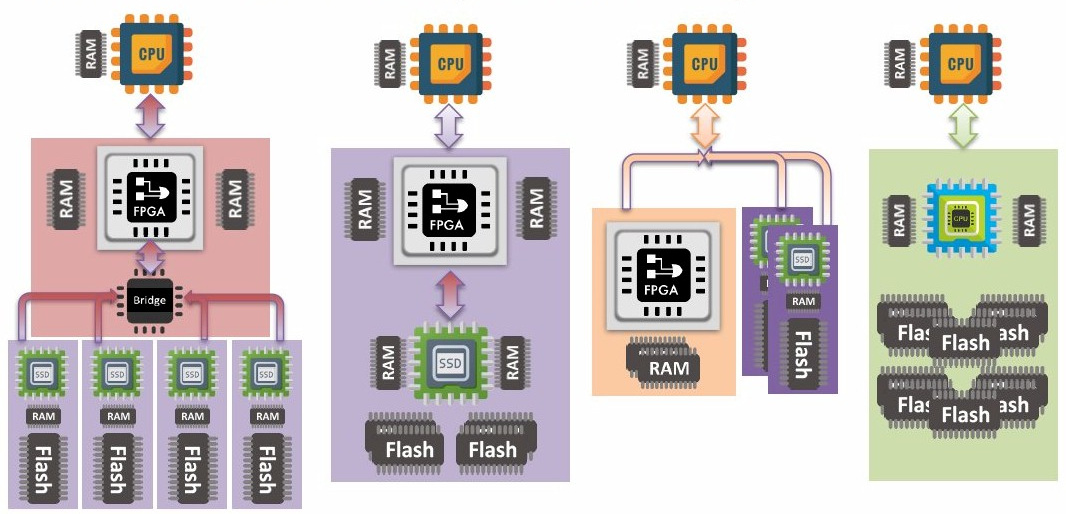
\includegraphics[width=1\textwidth]{resources/images/comp-stor2}
			\end{figure}
%		\end{column}
%	\end{columns}
	\textit{\tiny SNIA, Computational Storage Architecture and Programming
	Model 0.5\cite{snia-model}}
	\endgroup
\end{frame}

%\begin{frame}{When Computational Storage}
%	\begin{figure}
%	   \centering
%	   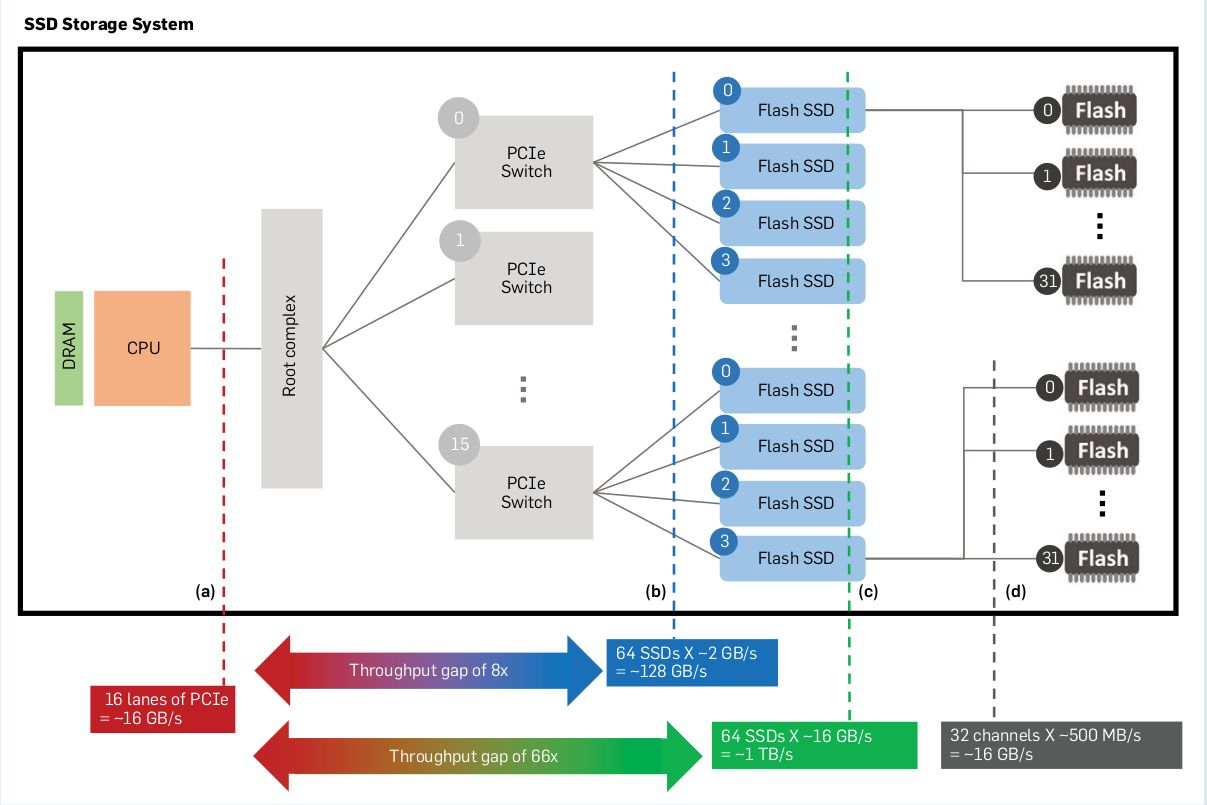
\includegraphics[width=0.8\textwidth]{resources/images/storage-gap}
%	\end{figure}
%	\begingroup
%	\textit{
%		\tiny Do, Jaeyoung, et al. Programmable solid-state storage in future
%		cloud datacenters\cite{do2019programmable}
%	}
%	\endgroup
%\end{frame}

\begin{frame}{Support Technologies}
	\begingroup
	\small % Figure of zoned storage
	\begin{figure}
	   \centering
	   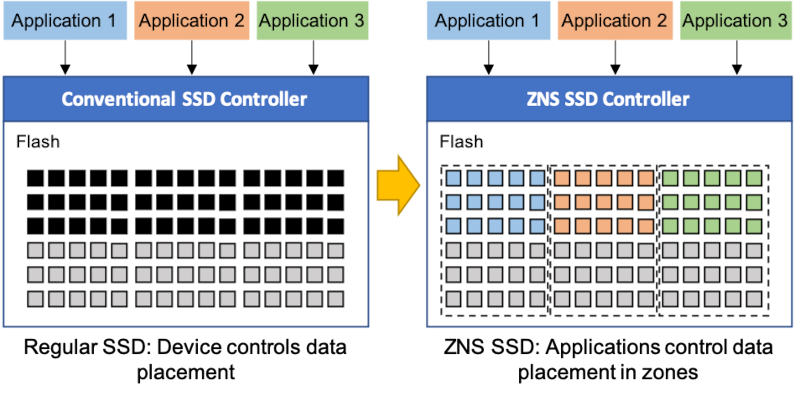
\includegraphics[width=0.8\textwidth]{resources/images/intro-zns}
	\end{figure}
	\textit{
		\tiny https://www.zonedstorage.io/introduction/zns/,
		Zoned Namespaces (ZNS) SSDs
	}
	\endgroup
\end{frame}

\begin{frame}{ZCSD}
	\begingroup
	\small An emulated programmable computational flash storage device
	\begin{figure}
		\centering
		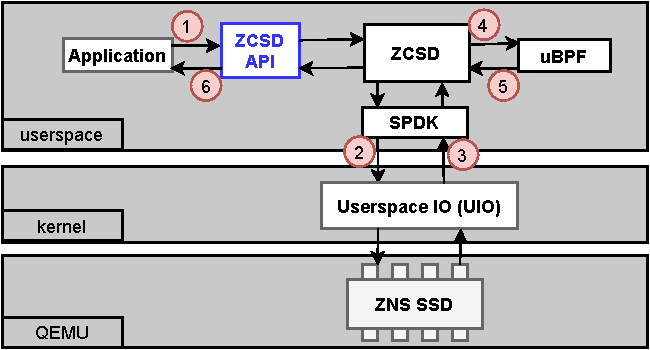
\includegraphics[width=0.8\textwidth]{resources/images/zcsd-arch-final}
	\end{figure}
	\endgroup
\end{frame}

\begin{frame}{}
	\begingroup
	\small
%	\begin{columns}
%		\begin{column}{0.4\textwidth}
%			\cexternal{resources/c/filter.c}
%		\end{column}
%		\begin{column}{0.6\textwidth}
			\begin{figure}
				\centering
				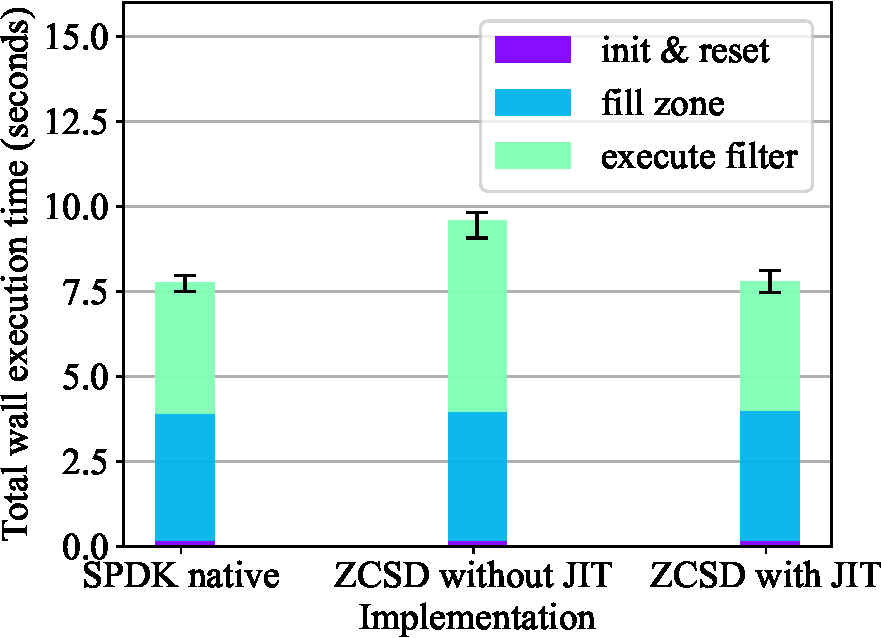
\includegraphics[width=0.9\textwidth]{resources/images/performance-crop}
			\end{figure}
%		\end{column}
%	\end{columns}
	\endgroup
\end{frame}

\begin{frame}{Whats next}
	\begingroup
	\small
	\begin{itemize}
		\item Many open research questions await.
		\begin{itemize}
			\item Handling abstractions, file systems / databases
			\item Safety, Security, Concurrency
			\item Energy efficiency \& Performance
			\item Implementability
			\item Autogeneration
			\item Ease of use, logging, debugging etc
		\end{itemize}
		\item We want you to use ZCSD \href{https://github.com/Dantali0n/qemu-csd}{https://github.com/Dantali0n/qemu-csd}
	\end{itemize}
	\endgroup
\end{frame}

\begin{frame}{References}
	\begingroup
	\tiny
	\bibliographystyle{plain}
	\bibliography{bibliography}
	\endgroup
\end{frame}

\end{document}